\documentclass[11pt,a4paper]{article}
\newcommand{\intestazione}{Trimero ad anello --- 10. VQE noise-aware}
% =====================================================================
%  Preambolo comune ai documenti sul dimero (serie "che cosa abbiamo fatto")
%  Incluso con % =====================================================================
%  Preambolo comune ai documenti sul dimero (serie "che cosa abbiamo fatto")
%  Incluso con % =====================================================================
%  Preambolo comune ai documenti sul dimero (serie "che cosa abbiamo fatto")
%  Incluso con \input{preambolo_dimero} subito dopo \documentclass.
% =====================================================================
\usepackage[T1]{fontenc}
\usepackage[utf8]{inputenc}
\usepackage[main=italian,provide=*]{babel}
\usepackage{amsmath,amssymb,mathtools}
\usepackage{graphicx}
\usepackage{booktabs}
\usepackage{colortbl}
\usepackage{xcolor}
\usepackage{geometry}
\usepackage{placeins}
\usepackage{caption}
\usepackage{enumitem}
\usepackage{fancyhdr}
\usepackage{needspace}
\usepackage{tikz}
\usetikzlibrary{arrows.meta,positioning,shapes.geometric,calc,fit,backgrounds}
\usepackage{hyperref}
\hypersetup{colorlinks=true,linkcolor=blu,citecolor=blu,urlcolor=blu}

\geometry{margin=2.5cm}

% --- colori coerenti con quelli delle figure (palette Okabe-Ito)
\definecolor{blu}{HTML}{0072B2}
\definecolor{arancio}{HTML}{E69F00}
\definecolor{verdes}{HTML}{009E73}
\definecolor{rossos}{HTML}{D55E00}
\definecolor{violas}{HTML}{CC79A7}
\definecolor{grigetto}{HTML}{E8E8E8}

\captionsetup{font=small,labelfont=bf,width=0.92\textwidth}

\pagestyle{fancy}
\fancyhf{}
\fancyhead[L]{\small\itshape\intestazione}
\fancyhead[R]{\small\thepage}
\renewcommand{\headrulewidth}{0.3pt}

% --- notazione
\newcommand{\ket}[1]{\lvert #1\rangle}
\newcommand{\bra}[1]{\langle #1 \rvert}
\newcommand{\media}[1]{\langle #1 \rangle}
\newcommand{\vs}[1]{\mathbf{s}_{#1}}

% --- riquadro "in una riga": il messaggio da portare a casa
\newcommand{\messaggio}[1]{%
  \begin{center}
  \begin{minipage}{0.93\textwidth}
  \setlength{\fboxsep}{9pt}%
  \colorbox{grigetto}{\begin{minipage}{\dimexpr\textwidth-2\fboxsep}
  \small\textbf{In una riga.}\enspace #1
  \end{minipage}}
  \end{minipage}
  \end{center}
}

% --- riquadro "come lo sappiamo": la verifica numerica dietro un'affermazione
\newcommand{\verifica}[1]{%
  \begin{center}
  \begin{minipage}{0.93\textwidth}
  \small\textcolor{verdes}{\rule{2.2em}{1.1pt}}\enspace
  \textcolor{verdes}{\textbf{Come lo sappiamo.}}\enspace #1
  \end{minipage}
  \end{center}
  \medskip
}
 subito dopo \documentclass.
% =====================================================================
\usepackage[T1]{fontenc}
\usepackage[utf8]{inputenc}
\usepackage[main=italian,provide=*]{babel}
\usepackage{amsmath,amssymb,mathtools}
\usepackage{graphicx}
\usepackage{booktabs}
\usepackage{colortbl}
\usepackage{xcolor}
\usepackage{geometry}
\usepackage{placeins}
\usepackage{caption}
\usepackage{enumitem}
\usepackage{fancyhdr}
\usepackage{needspace}
\usepackage{tikz}
\usetikzlibrary{arrows.meta,positioning,shapes.geometric,calc,fit,backgrounds}
\usepackage{hyperref}
\hypersetup{colorlinks=true,linkcolor=blu,citecolor=blu,urlcolor=blu}

\geometry{margin=2.5cm}

% --- colori coerenti con quelli delle figure (palette Okabe-Ito)
\definecolor{blu}{HTML}{0072B2}
\definecolor{arancio}{HTML}{E69F00}
\definecolor{verdes}{HTML}{009E73}
\definecolor{rossos}{HTML}{D55E00}
\definecolor{violas}{HTML}{CC79A7}
\definecolor{grigetto}{HTML}{E8E8E8}

\captionsetup{font=small,labelfont=bf,width=0.92\textwidth}

\pagestyle{fancy}
\fancyhf{}
\fancyhead[L]{\small\itshape\intestazione}
\fancyhead[R]{\small\thepage}
\renewcommand{\headrulewidth}{0.3pt}

% --- notazione
\newcommand{\ket}[1]{\lvert #1\rangle}
\newcommand{\bra}[1]{\langle #1 \rvert}
\newcommand{\media}[1]{\langle #1 \rangle}
\newcommand{\vs}[1]{\mathbf{s}_{#1}}

% --- riquadro "in una riga": il messaggio da portare a casa
\newcommand{\messaggio}[1]{%
  \begin{center}
  \begin{minipage}{0.93\textwidth}
  \setlength{\fboxsep}{9pt}%
  \colorbox{grigetto}{\begin{minipage}{\dimexpr\textwidth-2\fboxsep}
  \small\textbf{In una riga.}\enspace #1
  \end{minipage}}
  \end{minipage}
  \end{center}
}

% --- riquadro "come lo sappiamo": la verifica numerica dietro un'affermazione
\newcommand{\verifica}[1]{%
  \begin{center}
  \begin{minipage}{0.93\textwidth}
  \small\textcolor{verdes}{\rule{2.2em}{1.1pt}}\enspace
  \textcolor{verdes}{\textbf{Come lo sappiamo.}}\enspace #1
  \end{minipage}
  \end{center}
  \medskip
}
 subito dopo \documentclass.
% =====================================================================
\usepackage[T1]{fontenc}
\usepackage[utf8]{inputenc}
\usepackage[main=italian,provide=*]{babel}
\usepackage{amsmath,amssymb,mathtools}
\usepackage{graphicx}
\usepackage{booktabs}
\usepackage{colortbl}
\usepackage{xcolor}
\usepackage{geometry}
\usepackage{placeins}
\usepackage{caption}
\usepackage{enumitem}
\usepackage{fancyhdr}
\usepackage{needspace}
\usepackage{tikz}
\usetikzlibrary{arrows.meta,positioning,shapes.geometric,calc,fit,backgrounds}
\usepackage{hyperref}
\hypersetup{colorlinks=true,linkcolor=blu,citecolor=blu,urlcolor=blu}

\geometry{margin=2.5cm}

% --- colori coerenti con quelli delle figure (palette Okabe-Ito)
\definecolor{blu}{HTML}{0072B2}
\definecolor{arancio}{HTML}{E69F00}
\definecolor{verdes}{HTML}{009E73}
\definecolor{rossos}{HTML}{D55E00}
\definecolor{violas}{HTML}{CC79A7}
\definecolor{grigetto}{HTML}{E8E8E8}

\captionsetup{font=small,labelfont=bf,width=0.92\textwidth}

\pagestyle{fancy}
\fancyhf{}
\fancyhead[L]{\small\itshape\intestazione}
\fancyhead[R]{\small\thepage}
\renewcommand{\headrulewidth}{0.3pt}

% --- notazione
\newcommand{\ket}[1]{\lvert #1\rangle}
\newcommand{\bra}[1]{\langle #1 \rvert}
\newcommand{\media}[1]{\langle #1 \rangle}
\newcommand{\vs}[1]{\mathbf{s}_{#1}}

% --- riquadro "in una riga": il messaggio da portare a casa
\newcommand{\messaggio}[1]{%
  \begin{center}
  \begin{minipage}{0.93\textwidth}
  \setlength{\fboxsep}{9pt}%
  \colorbox{grigetto}{\begin{minipage}{\dimexpr\textwidth-2\fboxsep}
  \small\textbf{In una riga.}\enspace #1
  \end{minipage}}
  \end{minipage}
  \end{center}
}

% --- riquadro "come lo sappiamo": la verifica numerica dietro un'affermazione
\newcommand{\verifica}[1]{%
  \begin{center}
  \begin{minipage}{0.93\textwidth}
  \small\textcolor{verdes}{\rule{2.2em}{1.1pt}}\enspace
  \textcolor{verdes}{\textbf{Come lo sappiamo.}}\enspace #1
  \end{minipage}
  \end{center}
  \medskip
}

\providecommand{\Tr}{\operatorname{Tr}}

\title{\bfseries Vale la pena rioptimizzare vedendo il rumore?\\[2pt]
\large Documento 10 --- estensione facoltativa, un risultato diverso dal dimero}
\author{Samuele Schiavi \\ \small Tesi triennale in Fisica, Università di Parma
--- Relatore: Prof.\ Alessandro Chiesa}
\date{}

\begin{document}
\maketitle
\thispagestyle{fancy}

\section{La domanda complementare}

Punto di lavoro di tutto questo documento: \textbf{Scenario A} ($b/J=2.4$,
$D/J=0.15$, Opzione DM B) --- lo stesso dei Documenti 6--9. Il Documento 6
misura la degradazione di un VQE \emph{ideale} eseguito su
un simulatore rumoroso. Qui la domanda è diversa: se il rumore è acceso già
durante l'ottimizzazione --- come accadrebbe su hardware reale, dove non
esiste una versione ideale a cui accedere per calibrare --- l'ottimizzatore
converge a parametri diversi? E se sì, cambia qualcosa a valle?

\messaggio{Sul dimero la risposta era netta: nessun vantaggio misurabile,
verificato su due metriche, due punti di lavoro, l'intera griglia di
rumore. Qui la risposta è più ricca --- dipende da una scelta metodologica
che sul dimero non faceva differenza, e qui la fa.}

\section{L'argomento fisico, e una previsione prima di verificarla}

Per un canale depolarizzante isotropo,
$$E_\text{rumoroso}(\theta) = (1-\lambda)\,E_\text{ideale}(\theta) + \lambda\,\frac{\Tr[H]}{d},$$
trasformazione affine: lo stesso $\theta^*$ che minimizza $E_\text{ideale}$
minimizza anche $E_\text{rumoroso}$. Argomento generale, indipendente dal
sistema --- vale identico sul dimero e qui. \textbf{Previsione dichiarata
prima di guardare i numeri}: nessun vantaggio a rioptimizzare.

\section{Una scelta tecnica, scoperta lavorandoci}

L'argomento sopra presuppone una struttura di circuito fissa --- lo stesso
numero di gate rumorosi per qualunque $\theta$. Sul dimero questa premessa
è verificata banalmente (CNOT$=2$ su assegnazioni casuali). Qui \textbf{non
regge in generale}: con un ansatz a sei parametri, il transpilatore può
semplificare il blocco CNOT--$R_y(\theta)$--CNOT a valori speciali di
$\theta$ (vicini a $0$ o $\pi$), riducendo il conteggio CNOT.

\begin{figure}[htbp]
\centering
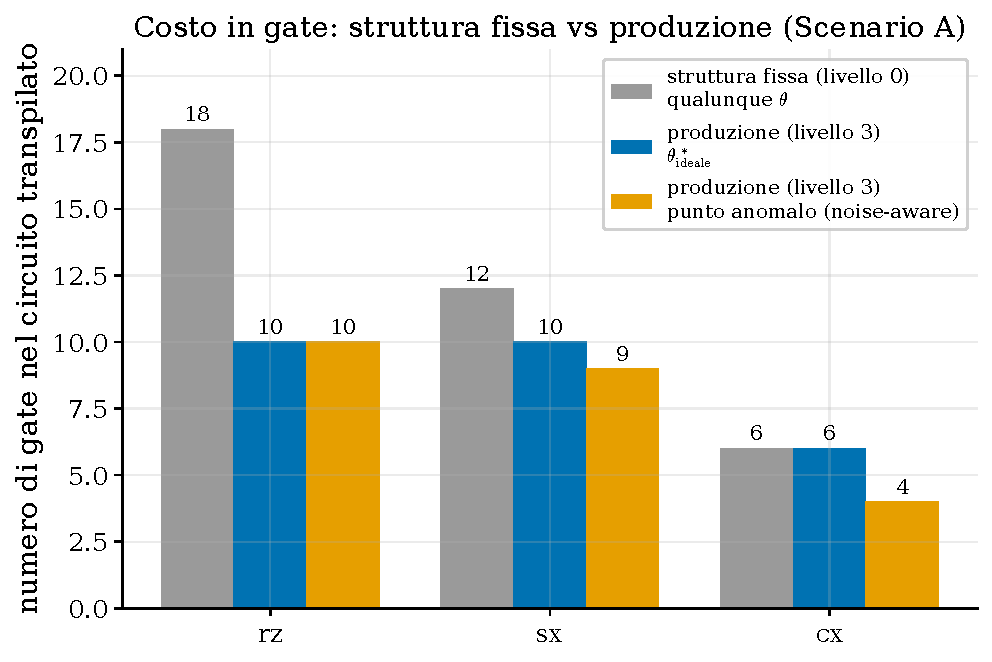
\includegraphics[width=0.72\textwidth]{figure/fig_bug_conteggio_gate_trimero_anello}
\caption{Costo in gate del circuito transpilato. A struttura fissa
(livello di ottimizzazione 0), sempre lo stesso conteggio qualunque
$\theta$. A produzione (livello 3), $\theta^*_\text{ideale}$ dà CNOT$=6$,
ma un punto trovato dall'ottimizzatore noise-aware (vicino a
$\theta_1{=}\pi,\theta_2{=}0$) dà CNOT$=4$.}
\end{figure}
\FloatBarrier

\verifica{Su 5 assegnazioni casuali di $\theta$, CNOT$=6$ sia a livello 0
sia a livello 3 --- il comportamento anomalo non è generico, emerge solo
quando l'ottimizzatore stesso trova valori speciali. A struttura fissa
(livello 0), verificato che il conteggio resta $6$ anche a quei valori
speciali.}

Per isolare l'effetto fisico da questo artefatto, tutto il resto di questo
documento usa la \textbf{struttura fissa} come metodologia principale; il
comportamento a struttura variabile (produzione) è riportato a parte, come
nota, non come risultato primario.

\section{Risultato 1: energia e fedeltà}

Multistart $R=12$ punti casuali $+1$ seme $=\theta^*_\text{ideale}$,
struttura fissa.

\begin{table}[htbp]
\centering
\small
\renewcommand{\arraystretch}{1.3}
\begin{tabular}{@{}lcc@{}}
\toprule
\rowcolor{grigetto}
\textbf{Quantità} & \textbf{riuso $\theta^*_\text{ideale}$} & \textbf{VQE noise-aware} \\
\midrule
$E$ (rumoroso) & $-5.36232432$ & $-5.36648903$ \\
$F$ (rumorosa) & $0.96728547$ & $0.95153755$ \\
CNOT & 6 & 6 \\
\bottomrule
\end{tabular}
\end{table}
\FloatBarrier

$\Delta E=-4.16\times10^{-3}$, $\Delta F=-1.57\times10^{-2}$ ---
\textbf{energia migliore, fedeltà peggiore}. Diverso, nella sostanza, dal
dimero ($\Delta E\sim10^{-7}$, $\Delta F>0$): qui la riottimizzazione trova
genuinamente un punto diverso, non rumore numerico attorno allo stesso
ottimo.

\messaggio{L'argomento affine garantisce solo che $\theta^*_\text{ideale}$
resta un minimo di $E_\text{ideale}$, non che sia l'unico minimo rilevante
di $E_\text{rumoroso}$ quando la dimensionalità cresce da tre a sei
parametri.}

\section{Robustezza del multistart}

\begin{figure}[htbp]
\centering
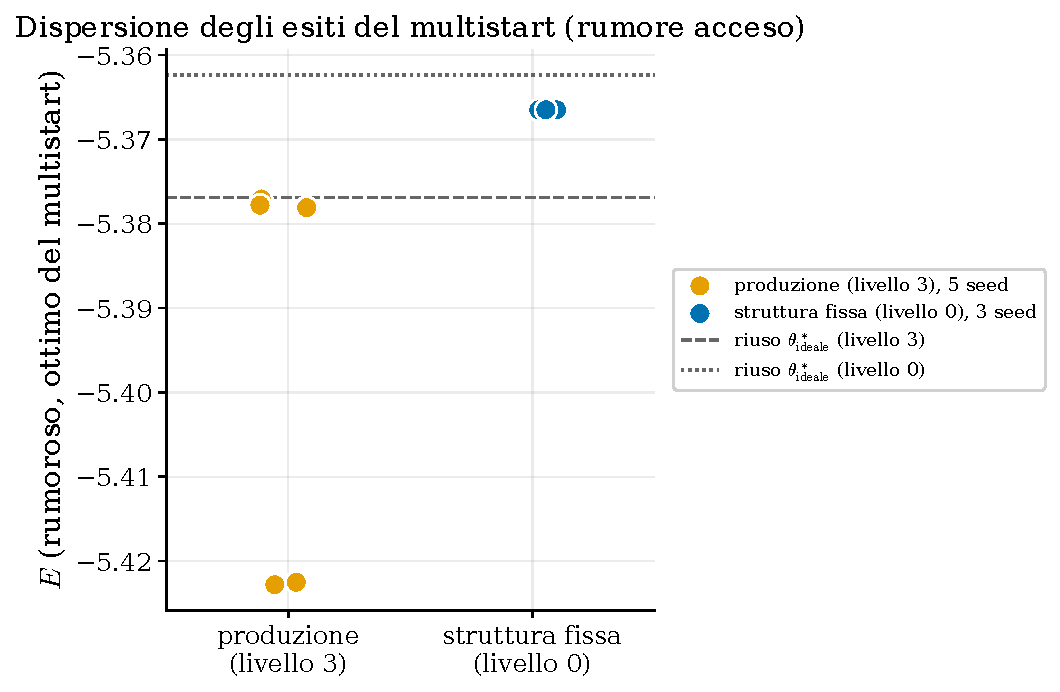
\includegraphics[width=0.72\textwidth]{figure/fig_robustezza_multistart_trimero_anello}
\caption{Dispersione degli esiti del multistart, 5 seed a livello 3
(produzione) contro 3 seed a livello 0 (struttura fissa). A struttura
fissa i tre punti sono sovrapposti; a produzione i cinque seed si separano
in due gruppi ben distinti.}
\end{figure}
\FloatBarrier

A struttura fissa, 3/3 seed convergono identici entro $2\times10^{-11}$.
A produzione, dispersione di $4.6\times10^{-2}$ in $E$: l'ottimizzatore sta
in parte esplorando artefatti del transpilatore, non solo la fisica.

\section{Risultato 2: $N^*$ della fedeltà di Trotter}

\begin{figure}[htbp]
\centering
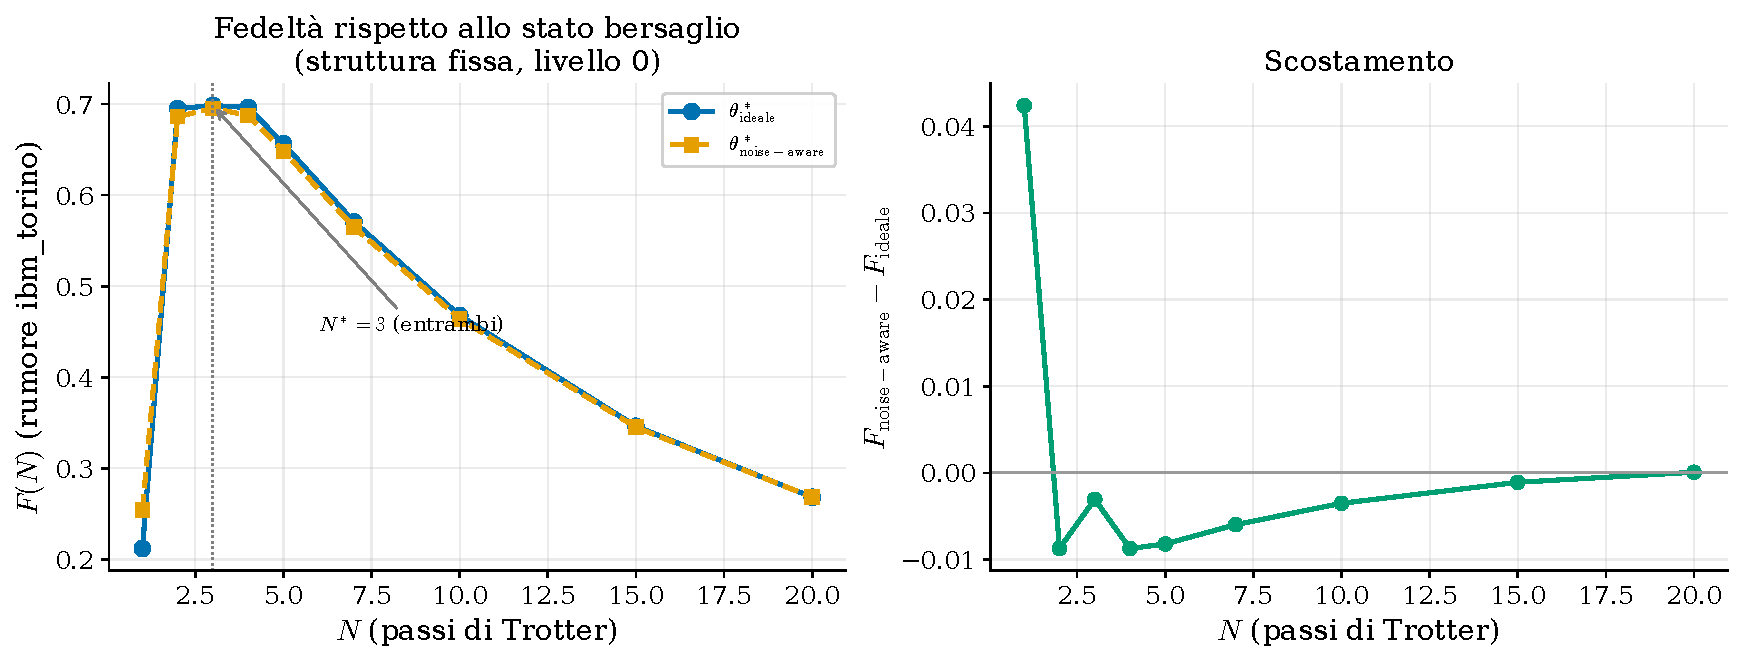
\includegraphics[width=\textwidth]{figure/fig_F_vs_N_confronto_trimero_anello}
\caption{Fedeltà di Trotter, struttura fissa. $N^*=3$ in entrambi i casi;
scostamento piccolo (scala $\sim10^{-2}$).}
\end{figure}
\FloatBarrier

$N^*=3$ invariato, coincide col baseline già noto.

\section{Risultato 3: $N^*$ del correlatore dinamico}

A differenza del Documento 6 (nessuna misura coinvolta), qui il readout
conta: verificato a \textbf{shot finiti}, non con la formula a operatore
densità usata nella prima verifica di questo controllo.

\begin{figure}[htbp]
\centering
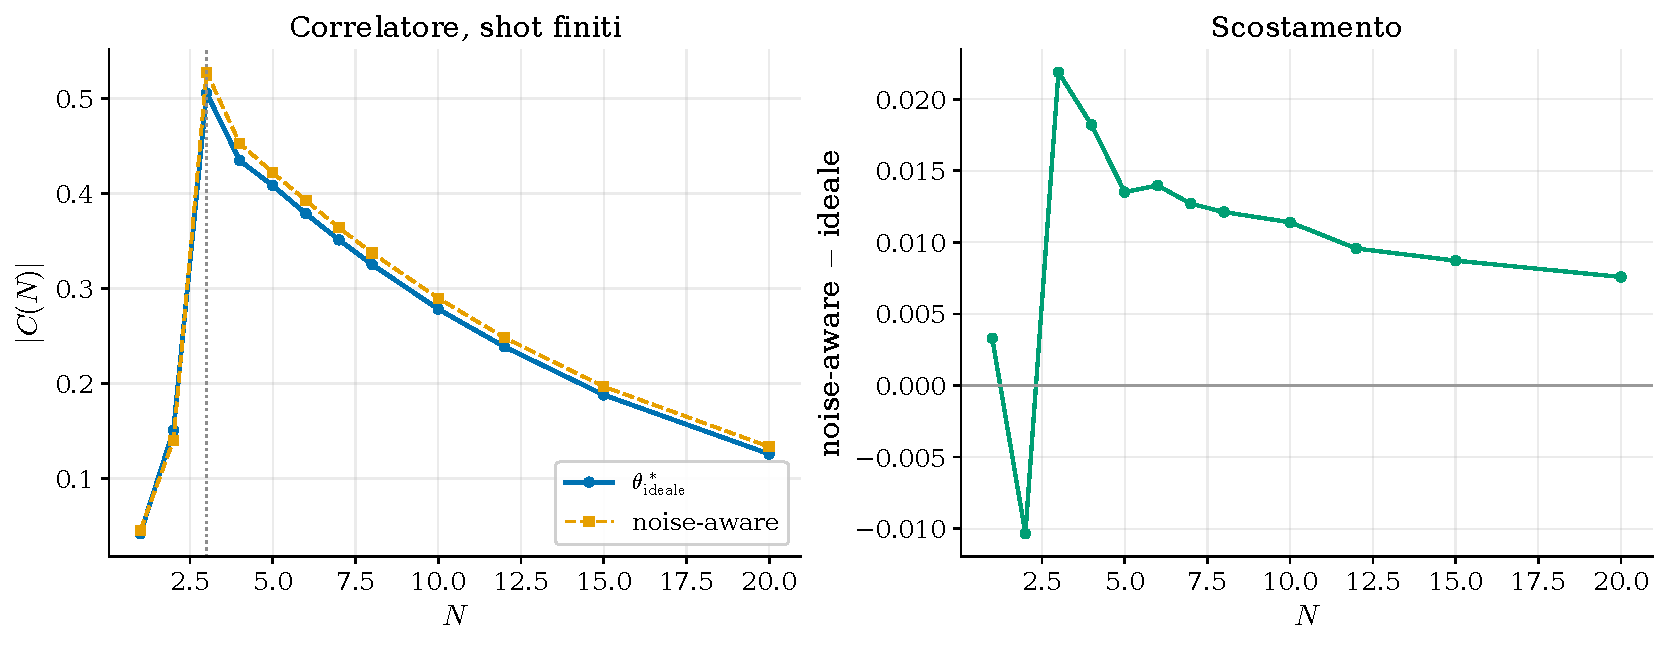
\includegraphics[width=\textwidth]{figure/fig_correlatore_noise_aware_confronto_anello_shots}
\caption{Modulo del correlatore, shot finiti ($8\times10^4$ shot per
punto). $N^*=3$ in entrambi i casi.}
\end{figure}
\FloatBarrier

\verifica{$N^*=3\to3$, coerente col risultato già ottenuto a operatore
densità esatto (stesso $N^*=3$) --- il passaggio a una misura vera non
cambia la conclusione, solo introduce l'attesa dispersione statistica sui
valori intermedi della curva.}

\section{Nota: cosa succede a struttura di produzione}

Ripetendo lo stesso controllo con la struttura variabile (il punto
anomalo, $4$ CNOT), l'esito è diverso e diverso fra le due metriche: $N^*$
Trotter si sposta ($3\to4$, scarto piccolo ma il massimo cambia
posizione), $N^*$ del correlatore no ($3\to3$).

\begin{figure}[htbp]
\centering
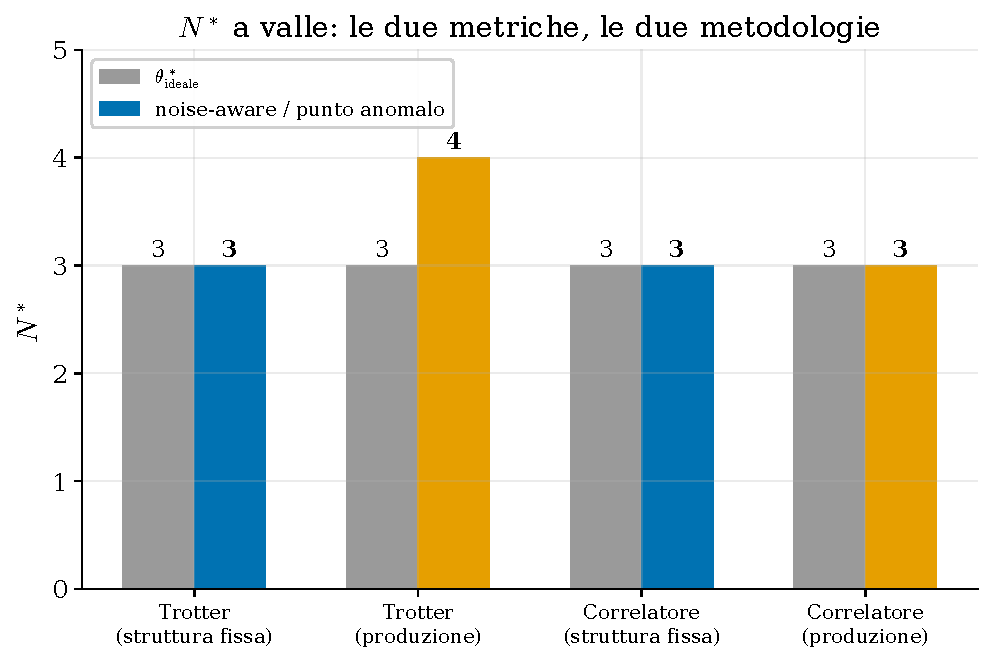
\includegraphics[width=0.68\textwidth]{figure/fig_Nstar_confronto_metodologie_trimero_anello}
\caption{$N^*$ a valle, le due metriche e le due metodologie a confronto.}
\end{figure}
\FloatBarrier

\messaggio{Questa nota non invalida il risultato principale: mostra che la
pipeline di produzione, usata senza accorgimenti per un'estensione
noise-aware su un ansatz a più parametri, può restituire conclusioni
dipendenti da un artefatto del transpilatore --- una lezione metodologica,
non solo per questa estensione.}

\section{Perché l'argomento di continuità del dimero non si applica qui}

Sul dimero, l'invarianza di $N^*$ era spiegata da un argomento di
continuità: $\theta^*_\text{noise-aware}$ quasi indistinguibile da
$\theta^*_\text{ideale}$, quindi qualunque osservabile liscio a valle
differisce di una quantità altrettanto minuscola. Qui $\lVert\Delta\theta
\rVert$ \textbf{non è piccolo} --- $\Delta E$ e $\Delta F$ sono tre ordini
di grandezza più grandi del dimero. Che $N^*$ resti comunque invariato non
è quindi spiegato dalla piccolezza di $\Delta\theta$, ma da un fatto più
debole: l'osservabile a valle è sufficientemente insensibile a
\emph{questo particolare} $\Delta\theta$, non a un $\Delta\theta$ generico
--- non generalizza automaticamente ad altri punti di lavoro.

\section{Considerazioni}

\begin{itemize}[leftmargin=1.6em,itemsep=3pt]
\item Il risultato principale è diverso da quello del dimero, non solo più
complicato: qui la riottimizzazione produce un compromesso energia/fedeltà
reale, che però non si traduce in uno spostamento di $N^*$ a valle.
\item La scelta metodologica (struttura fissa contro produzione) qui non è
un dettaglio implementativo: sul dimero era irrilevante, qui determina se
si osserva un fenomeno fisico pulito o un artefatto del transpilatore
mescolato alla fisica.
\item Verificato a un solo punto di lavoro (Scenario A); non ripetuto a
$R_0$, che nella pipeline attuale non ha una preparazione VQE da
riottimizzare.
\end{itemize}

\end{document}
